\documentclass[11pt,a4paper]{article}

\usepackage[T1]{fontenc}
\usepackage[utf8]{inputenc}
\usepackage[ngerman]{babel}
\usepackage{lmodern}
\usepackage{microtype}
\usepackage[a4paper,margin=2.2cm,headheight=14pt]{geometry}
\usepackage{amsmath,amssymb,mathtools}
\usepackage{siunitx}
\usepackage{graphicx}
\usepackage{booktabs}
\usepackage{array}
\usepackage{float}
\usepackage{caption}
\usepackage{subcaption}
\usepackage{xcolor}
\usepackage{hyperref}
\usepackage{fancyhdr}
\usepackage{enumitem}

\definecolor{blue}{HTML}{1F4E79}
\definecolor{lightblue}{HTML}{EAF2F8}
\definecolor{gray}{HTML}{566573}

\hypersetup{
  colorlinks=true,
  linkcolor=blue,
  urlcolor=blue,
  citecolor=blue,
  pdftitle={Exercise 4 -- Orbits and Rocket Launch},
  pdfauthor={Computational Physics}
}

\sisetup{
  locale = DE,
  per-mode = symbol,
  exponent-product = \cdot,
  range-phrase = {--},
  range-units = single
}

\pagestyle{fancy}
\fancyhf{}
\lhead{\small Computational Physics -- Exercise 4}
\rhead{\small Orbits and Rocket Launch}
\cfoot{\thepage}

\setlength{\parindent}{0pt}
\setlength{\parskip}{0.55em}
\captionsetup{font=small,labelfont=bf,justification=centering}
\newcommand{\vect}[1]{\boldsymbol{#1}}
\newcommand{\code}[1]{\texttt{#1}}
\newcommand{\outputdir}{exercise\_04\_task\_}

\title{\textcolor{blue}{Exercise 4}\\[0.35em]
\large Symplektische Integratoren für Bahnen und Raketenstarts}
\author{Computational Physics}
\date{WS 2026/27}

\begin{document}

\maketitle
\thispagestyle{empty}

\begin{abstract}
Dieser Bericht fasst die Aufgaben 1 und 2 des Übungsblatts zusammen. Neben den
Modellgleichungen werden die verwendeten numerischen Verfahren, die
Erhaltungsgrößen und die physikalische Interpretation der Simulationen
erklärt. Die Abbildungen und Tabellen stammen aus den zugehörigen
Python-Skripten und dienen jeweils als direkte Kontrolle der theoretischen
Aussagen.
\end{abstract}

\tableofcontents
\newpage

\section{Verwendete Modelle und Konstanten}

Alle Rechnungen erfolgen in SI-Einheiten. Für die Erde werden
\[
G=\SI{6.674e-11}{\meter^3\kilogram^{-1}\second^{-2}},
\qquad
M_{\mathrm E}=\SI{5.972e24}{\kilogram},
\qquad
\mu=GM_{\mathrm E}
\]
verwendet. Die numerischen Verfahren sind in den wiederverwendbaren Modulen
\code{ode\_methods.py} und \code{rocket\_model.py} implementiert. Die beiden
Auswertungsskripte erzeugen die Abbildungen und CSV-Dateien im Ordner
\code{exercise\_04}.

\section{Aufgabe 1: Mondbahn um die Erde}

\subsection{1a: Kreisbahn und Anfangsbedingungen}

Die Erde wird als ruhender Punkt im Ursprung betrachtet. Die Bewegung des
Mondes wird durch
\begin{equation}
  \ddot{\vect r}
  =-\frac{GM_{\mathrm E}}{\lvert\vect r\rvert^3}\vect r
\end{equation}
beschrieben. Für eine Kreisbahn mit Radius $r_{\mathrm M}$ muss die
Gravitationsbeschleunigung der Zentripetalbeschleunigung entsprechen:
\begin{equation}
  \frac{v_{\mathrm M}^2}{r_{\mathrm M}}
  =\frac{GM_{\mathrm E}}{r_{\mathrm M}^2},
  \qquad
  v_{\mathrm M}=\sqrt{\frac{GM_{\mathrm E}}{r_{\mathrm M}}}.
\end{equation}

Mit dem Startpunkt auf der positiven $x$-Achse und einer Bewegung gegen den
Uhrzeigersinn werden die Anfangswerte
\[
\vect r(0)=
\begin{pmatrix}r_{\mathrm M}\\0\end{pmatrix},
\qquad
\vect v(0)=
\begin{pmatrix}0\\v_{\mathrm M}\end{pmatrix}
\]
verwendet. Die ideale Kepler-Periode lautet
\begin{equation}
  T=2\pi\sqrt{\frac{r_{\mathrm M}^3}{GM_{\mathrm E}}}.
\end{equation}

\begin{table}[H]
\centering
\caption{Anfangswerte und ideale Umlaufzeit.}
\begin{tabular}{@{}lr@{}}
\toprule
Größe & Wert\\
\midrule
$r_{\mathrm M}$ & \SI{3.84400e8}{\meter}\\
$v_{\mathrm M}$ & \SI{1.018266e3}{\meter\per\second}\\
$T$ aus dem Punktmassenmodell & \SI{27.452898}{\day}\\
siderischer Monat & \SI{27.32}{\day}\\
\bottomrule
\end{tabular}
\end{table}

Die Differenz zwischen der idealen Periode und dem siderischen Monat entsteht
nicht durch einen Fehler in der Herleitung. Das reale Erde--Mond-System ist
kein festes Erde-Punktmasse-Modell: Die Erde bewegt sich um das Baryzentrum,
die Mondbahn ist leicht exzentrisch und insbesondere die Sonne verursacht
merkliche Störungen. Zusätzlich sind die im Blatt vorgegebenen Konstanten und
der mittlere Mondradius gerundet.

\subsection{1b: Numerische Integratoren}

Verglichen werden expliziter Euler, impliziter Euler, Heun, symplektischer
Euler und Velocity-Verlet. Die Schrittweite beträgt $\Delta t=\SI{6}{\hour}$;
dargestellt sind zehn Umläufe.

Für den impliziten Euler-Schritt wird
\begin{equation}
  \vect y_{n+1}
  =\vect y_n+\Delta t\,\vect f(t_{n+1},\vect y_{n+1})
\end{equation}
mit Newtons Methode gelöst. Als Startwert wird ein expliziter Euler-Schritt
verwendet. Bei dieser groben Schrittweite verliert die implizite Bahn nach
etwa \SI{14.5}{\day} so viel Radius, dass die Punktmassensingularität
erreicht wird; das Skript meldet diesen Abbruch ausdrücklich.

\begin{figure}[H]
\centering
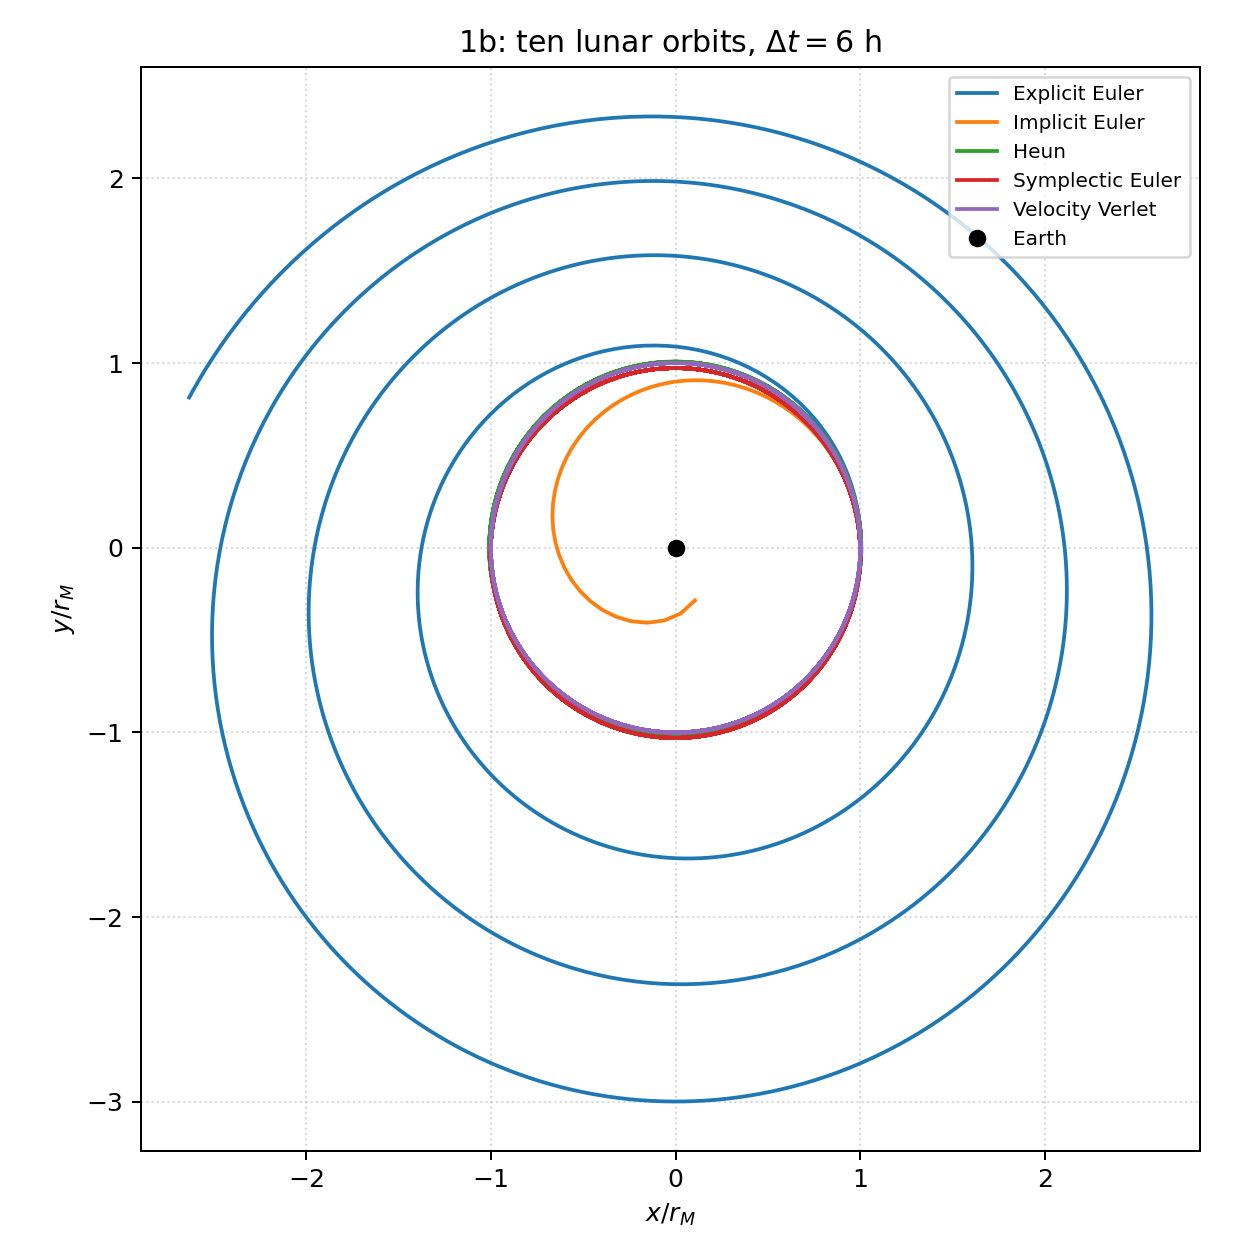
\includegraphics[width=0.76\textwidth]{exercise_04_task_1_output/task_1b_orbits.png}
\caption{Mondbahnen über zehn Umläufe bei $\Delta t=\SI{6}{\hour}$.}
\label{fig:moon-orbits}
\end{figure}

Expliziter Euler gewinnt Energie und spiralt nach außen. Impliziter Euler
verliert Energie und spiralt nach innen. Heun besitzt zwar Ordnung zwei, ist
aber nicht symplektisch; über viele Umläufe kann sich der kleine Energie- und
Phasenfehler daher aufsummieren. Symplektischer Euler und Velocity-Verlet
zeigen dagegen eine qualitativ gebundene Bahn mit beschränkten Fehlern.

\subsection{1c: Energie und Drehimpuls}

Die spezifische Energie und der spezifische Drehimpuls sind
\begin{equation}
  E=\frac{1}{2}\lvert\vect v\rvert^2-\frac{GM_{\mathrm E}}{\lvert\vect r\rvert},
  \qquad
  \vect L=\vect r\times\vect v.
\end{equation}
Mit $\dot{\vect r}=\vect v$ und
$\dot{\vect v}=-GM_{\mathrm E}\vect r/\lvert\vect r\rvert^3$ folgt
\begin{align}
  \frac{\mathrm dE}{\mathrm dt}
  &=\vect v\cdot\dot{\vect v}
    +\frac{GM_{\mathrm E}}{\lvert\vect r\rvert^2}
      \frac{\vect r\cdot\vect v}{\lvert\vect r\rvert}
   =0,\\
  \frac{\mathrm d\vect L}{\mathrm dt}
  &=\dot{\vect r}\times\vect v+\vect r\times\dot{\vect v}
   =\vect v\times\vect v
    -\frac{GM_{\mathrm E}}{\lvert\vect r\rvert^3}
      \vect r\times\vect r
   =0.
\end{align}

\begin{figure}[H]
\centering
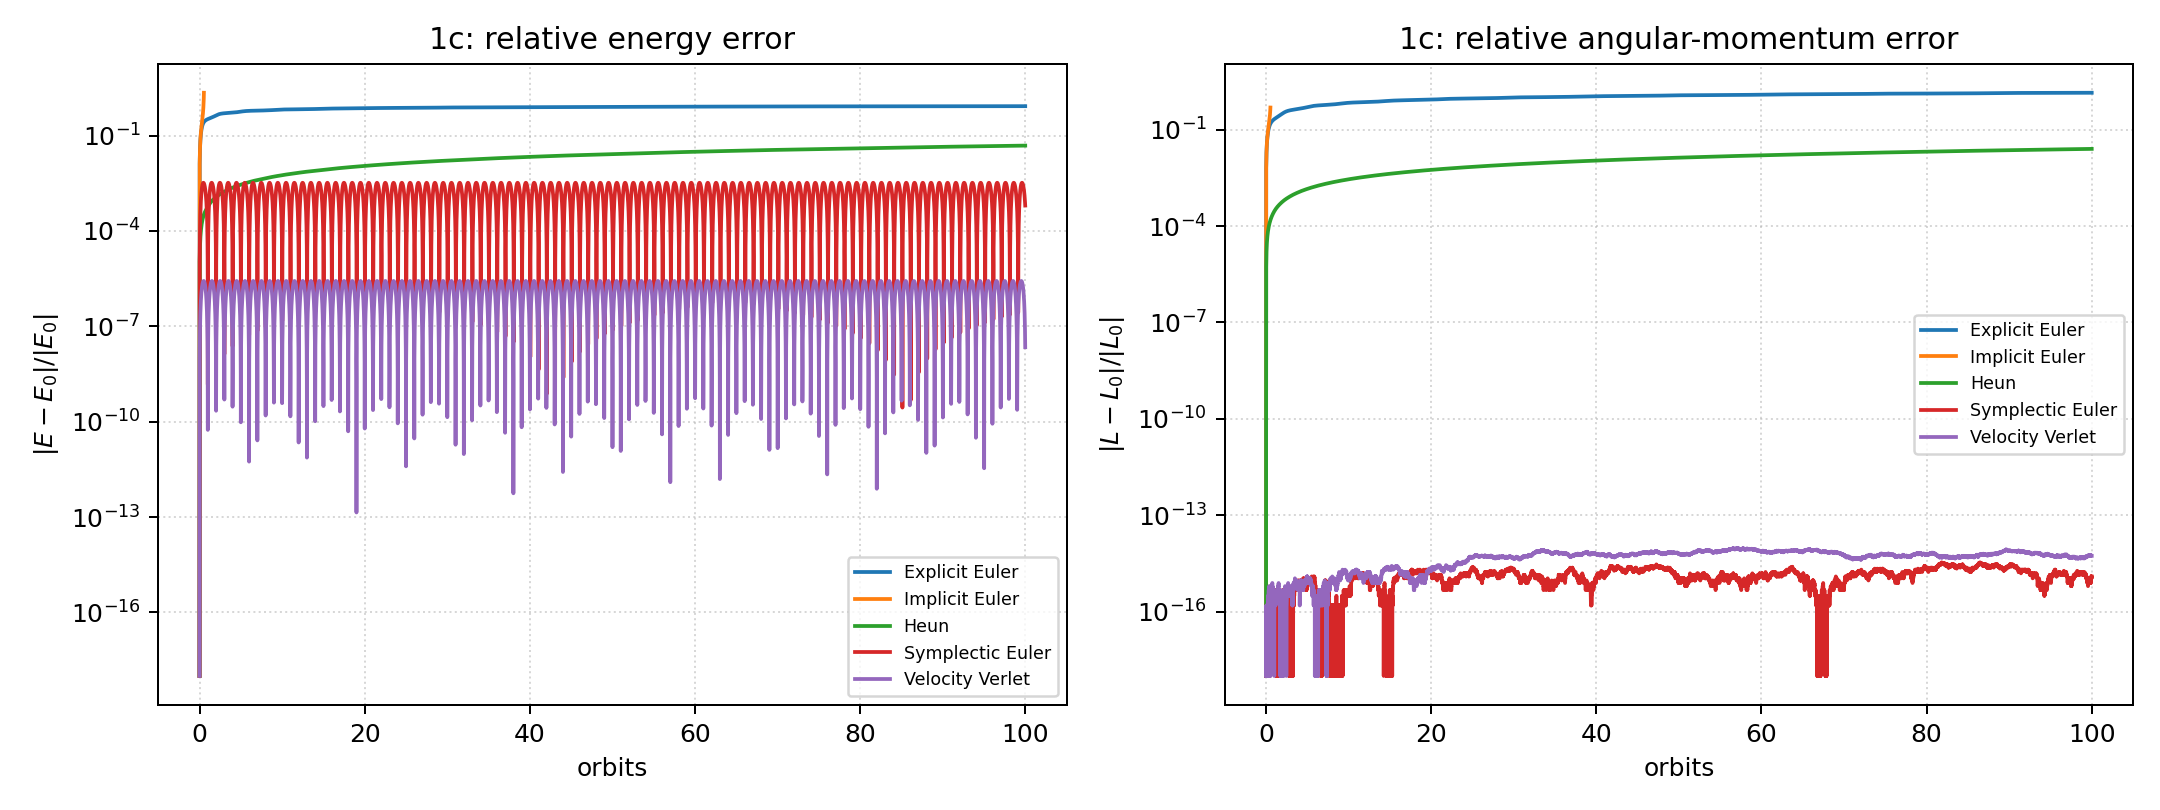
\includegraphics[width=\textwidth]{exercise_04_task_1_output/task_1c_invariants.png}
\caption{Relative Fehler der Energie und des Drehimpulses über 100 Umläufe.}
\label{fig:invariants}
\end{figure}

Für die zentrale Kraft erhält der velocity-first symplektische Euler-Schritt
den skalaren Drehimpuls exakt: Die Geschwindigkeitsänderung ist parallel zu
$\vect r_n$, und anschließend wird die Position mit $\vect v_{n+1}$ aktualisiert.
Symplektizität garantiert allerdings nicht die exakte Erhaltung jeder
Erhaltungsgröße. Ihr Vorteil liegt hier vor allem im beschränkten
Langzeitverhalten der Energie.

\subsection{1d: Konvergenz am halben Umlauf}

Zum Zeitpunkt $t=T/2$ ist die exakte Position
\[
\vect r(T/2)=(-r_{\mathrm M},0).
\]
Der Fehler wurde für
$\Delta t=T/200,\ldots,T/6400$ bestimmt. Die Steigung im log-log-Diagramm
entspricht der beobachteten Konvergenzordnung.

\begin{figure}[H]
\centering
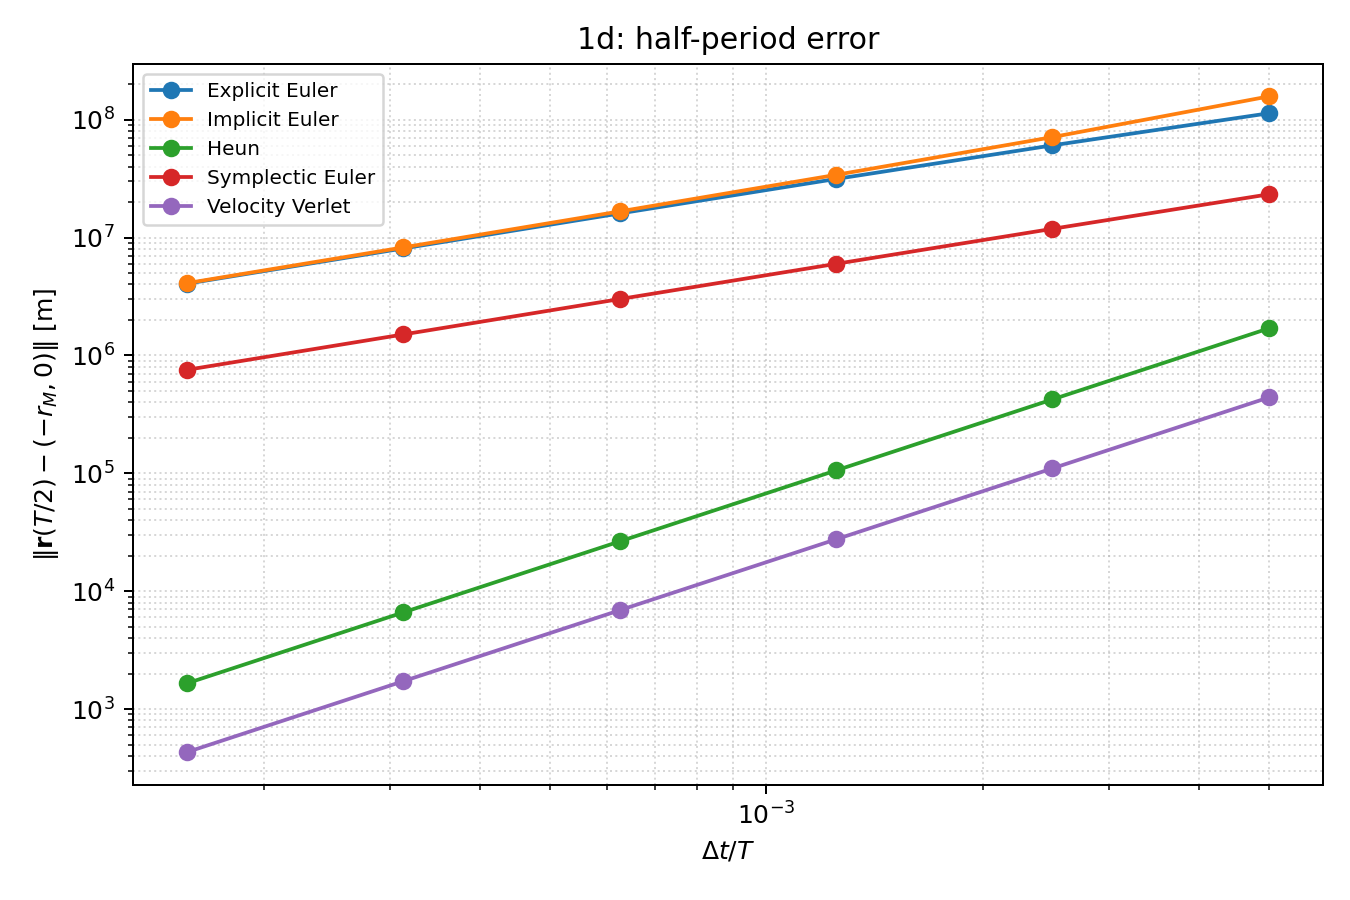
\includegraphics[width=0.78\textwidth]{exercise_04_task_1_output/task_1d_convergence.png}
\caption{Fehler bei $t=T/2$ für verschiedene Schrittweiten.}
\label{fig:convergence}
\end{figure}

\begin{table}[H]
\centering
\caption{Gemessene Konvergenzsteigungen.}
\begin{tabular}{@{}lr@{}}
\toprule
Verfahren & Steigung\\
\midrule
Expliziter Euler & 0.963\\
Impliziter Euler & 1.048\\
Heun & 2.001\\
Symplektischer Euler & 0.991\\
Velocity-Verlet & 2.000\\
\bottomrule
\end{tabular}
\end{table}

Für eine Simulation über \SI{1000}{\year} würde ich Velocity-Verlet wählen:
Das Verfahren ist zweiter Ordnung und besitzt für autonome Probleme gute
Langzeiteigenschaften. Die konkrete Schrittweite muss zusätzlich anhand des
zulässigen Phasenfehlers bestimmt werden.

\newpage
\section{Aufgabe 2: Raketenstart}

\subsection{Modell und Anfangszustand}

Die Rakete startet am Äquator mit der Rotationsgeschwindigkeit der Erde:
\[
\vect r(0)=
\begin{pmatrix}R_{\mathrm E}\\0\end{pmatrix},
\qquad
\vect v(0)=
\begin{pmatrix}0\\\omega_{\mathrm E}R_{\mathrm E}\end{pmatrix}.
\]
Während des Brennens gilt
\begin{equation}
  \ddot{\vect r}
  =-\frac{GM_{\mathrm E}}{\lvert\vect r\rvert^3}\vect r
   +\frac{F}{m(t)}\vect e(t),
  \qquad
  m(t)=m_0-\dot m\,t,
  \qquad
  F=\dot m\,v_e.
\end{equation}
Die rechte Seite wird mit klassischem RK4 integriert. Für die vertikale Studie
wird $\Delta t=\SI{0.5}{\second}$, für längere Trajektorien
$\Delta t=\SI{1}{\second}$ verwendet.

\subsection{2a: Vertikaler Start}

Bei $\theta=90^\circ$ ist $\vect e=\vect e_r$. Für $m_1=m_0/19$ ergibt sich
die Brenndauer
\begin{equation}
  t_b=\frac{m_0-m_1}{\dot m}
  =\left(1-\frac{1}{19}\right)\frac{v_e}{F/m_0}.
\end{equation}
Die ideale Raketengleichung liefert
\begin{equation}
  \Delta v_{\mathrm{ideal}}
  =v_e\ln\left(\frac{m_0}{m_1}\right)
  =\SI{4.4}{\kilo\meter\per\second}\ln(19)
  =\SI{12.956}{\kilo\meter\per\second}.
\end{equation}

\begin{figure}[H]
\centering
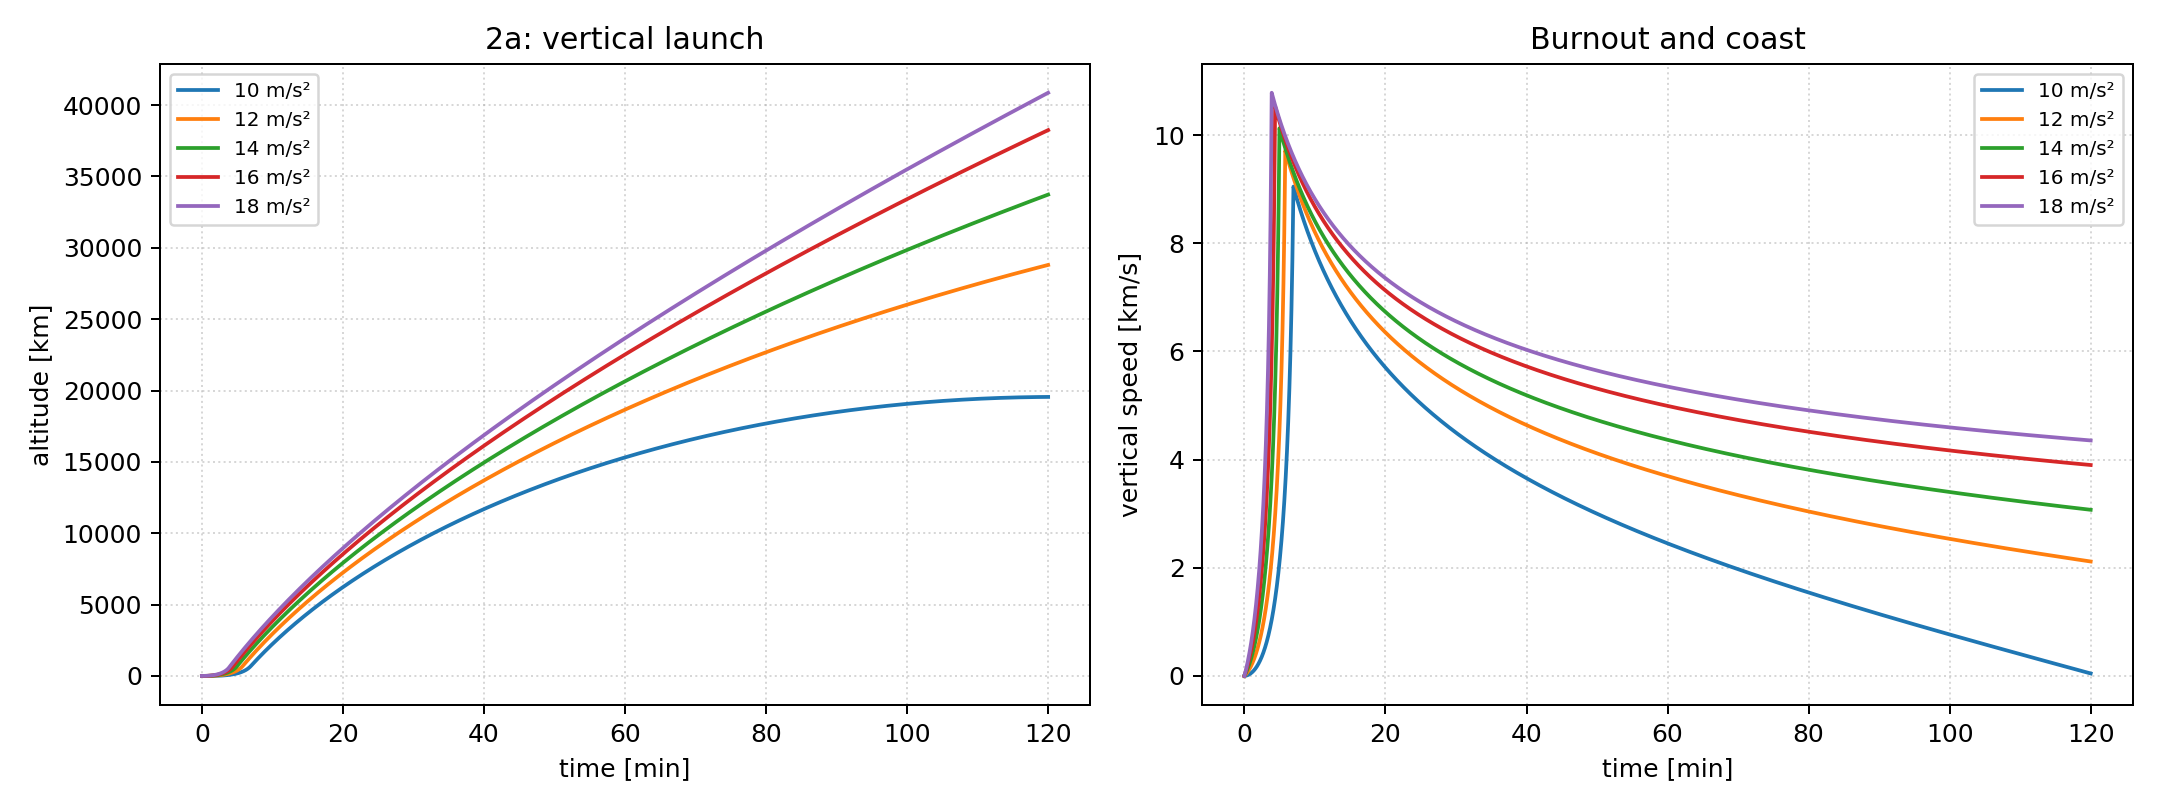
\includegraphics[width=\textwidth]{exercise_04_task_2_output/task_2a_vertical_launch.png}
\caption{Höhe und vertikale Geschwindigkeit für verschiedene Anfangsschübe.}
\label{fig:vertical}
\end{figure}

\begin{table}[H]
\centering
\caption{Vertikaler Start: Zustand bei Brennschluss.}
\small
\begin{tabular}{@{}rrrr@{}}
\toprule
$F/m_0$ [\si{\meter\per\second^2}] &
$t_b$ [\si{\second}] &
$v_b$ [\si{\kilo\meter\per\second}] &
$E_b$ [\si{\mega\joule\per\kilogram}]\\
\midrule
10 & 416.8 & 9.048 & $-15.368$\\
12 & 347.4 & 9.715 & $-9.090$\\
14 & 297.7 & 10.127 & $-5.218$\\
16 & 260.5 & 10.531 & $-1.326$\\
18 & 231.6 & 10.783 & $+1.044$\\
\bottomrule
\end{tabular}
\end{table}

Die Differenz zur idealen Raketengleichung entsteht hauptsächlich durch den
Gravitationsverlust während des Brennens. Bei den getesteten Werten ist
$F/m_0=\SI{18}{\meter\per\second^2}$ der erste Wert mit $E_b\geq0$. Ein
vertikaler Start kann keine Kreisbahn erzeugen, da am Brennschluss nahezu die
gesamte Geschwindigkeit radial gerichtet ist; eine Umlaufbahn benötigt
dagegen eine passende tangentiale Geschwindigkeit.

\subsection{2b: Pitch-Programm}

Die Schubrichtung lautet
\begin{equation}
  \vect e=\sin(\theta)\vect e_r
  \mathbin{\pm}\cos(\theta)\vect e_\phi,
  \qquad
  \theta(t)=90^\circ\max\left(0,1-\frac{t}{t_p}\right).
\end{equation}
Ein ostwärtiger Start nutzt die vorhandene Rotationsgeschwindigkeit der Erde.
Für die untersuchten Werte $t_p=100,125,\ldots,300\,\si{\second}$ werden
ostwärts die Fälle $t_p=150,175,200\,\si{\second}$ als gebundene Orbits
klassifiziert. Westwärts stürzen in diesem Raster alle Fälle ab.

\begin{figure}[H]
\centering
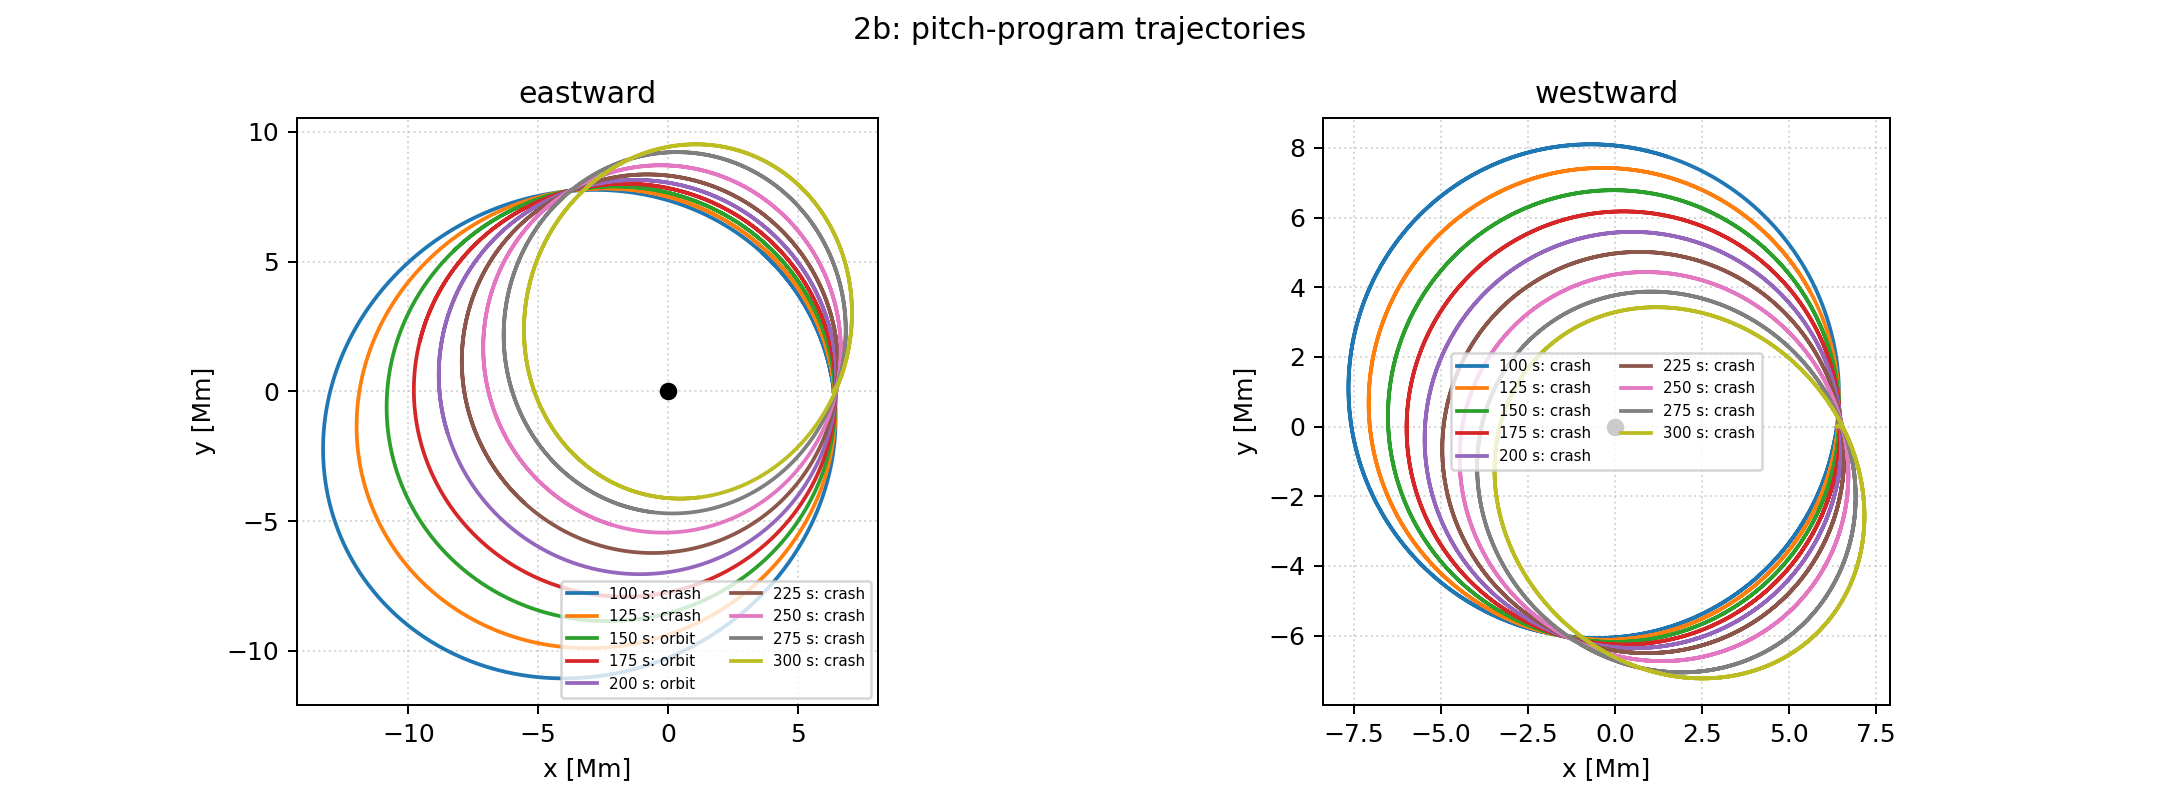
\includegraphics[width=\textwidth]{exercise_04_task_2_output/task_2b_pitch_program.png}
\caption{Trajektorien des Pitch-Programms für ost- und westwärtigen Start.}
\label{fig:pitch}
\end{figure}

\subsection{2c: Kreisbahnen durch Circularization}

Ein einzelner Brennvorgang endet im Allgemeinen auf einer Ellipse. Daher wird
die Rakete zunächst bis zum gewünschten Radius geflogen und anschließend die
Geschwindigkeit auf
\begin{equation}
  v_{\mathrm{circ}}=\sqrt{\frac{GM_{\mathrm E}}{R_{\mathrm E}+h}}
\end{equation}
korrigiert. Der zusätzliche Impuls ist
$\Delta\vect v=\vect v_{\mathrm{circ}}-\vect v$. Danach wird die Bewegung
ohne Schub weiter simuliert.

\begin{figure}[H]
\centering
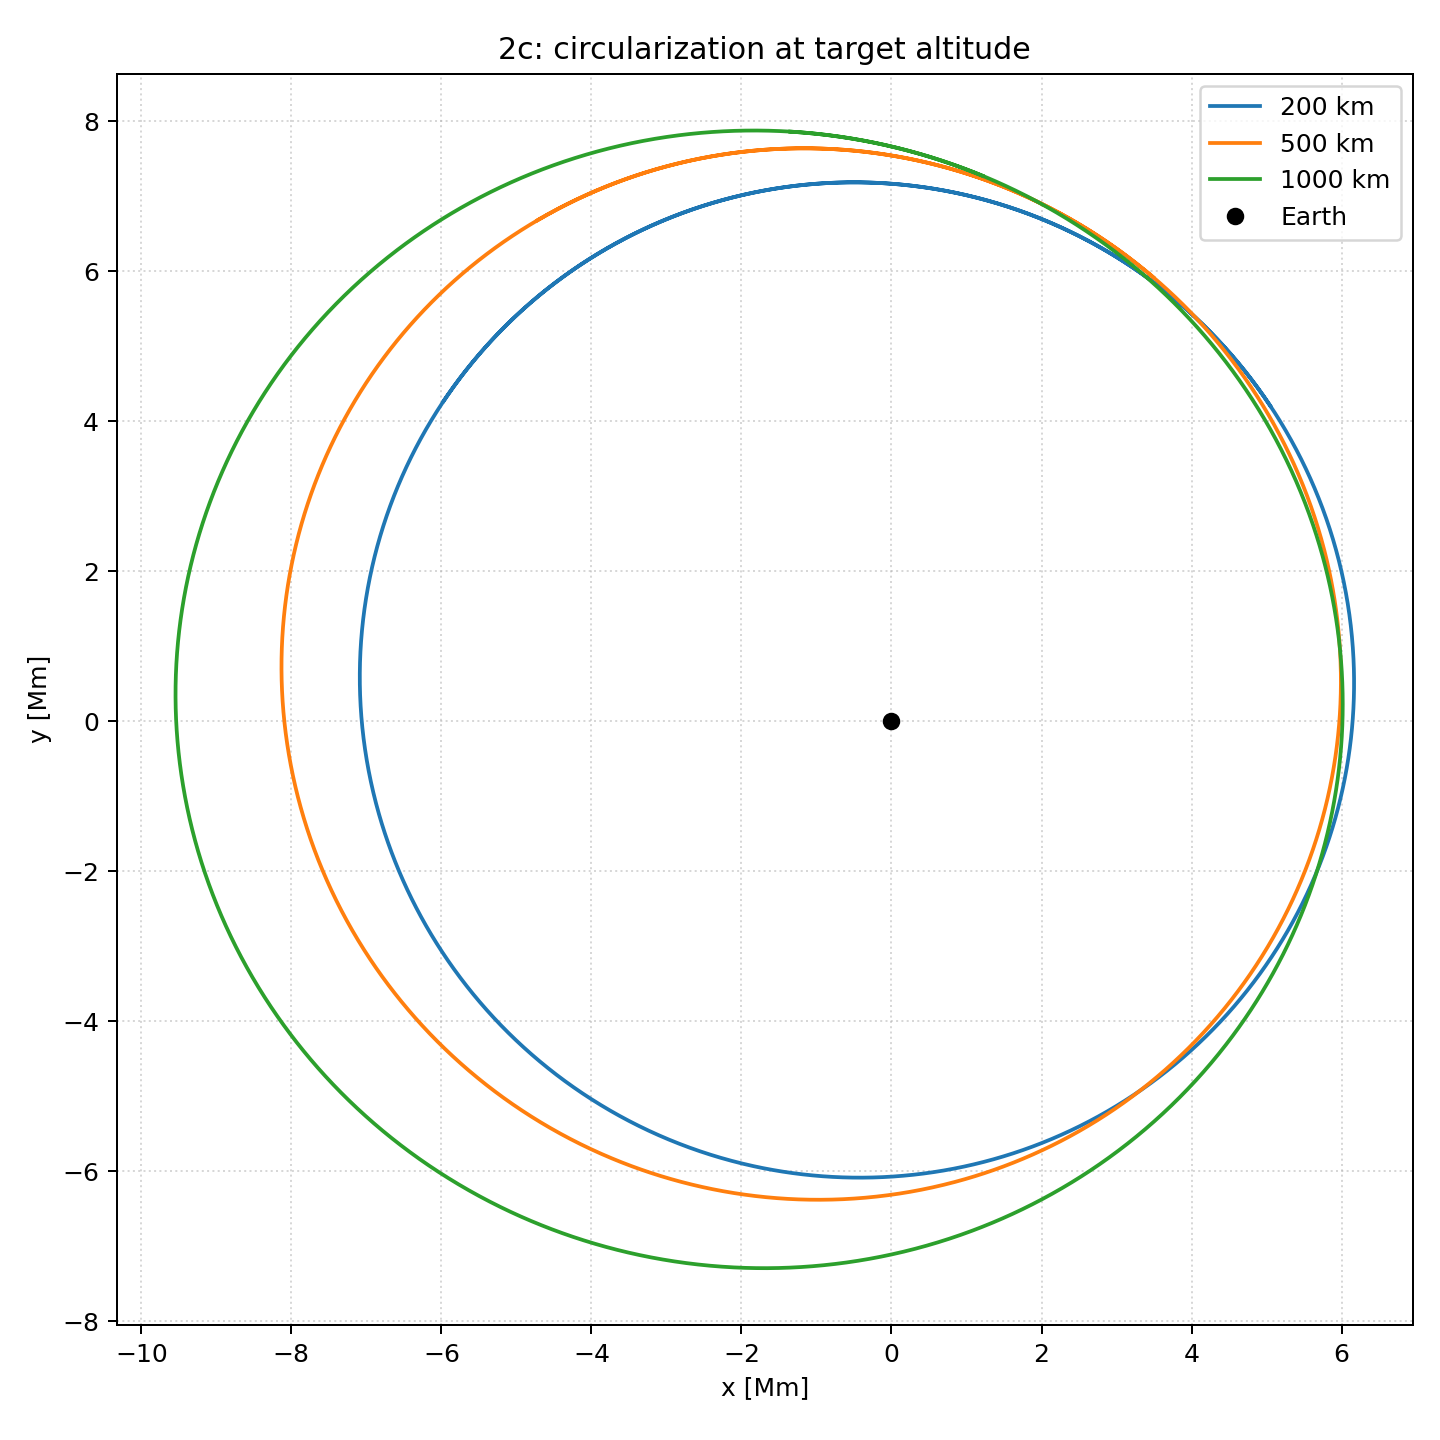
\includegraphics[width=0.78\textwidth]{exercise_04_task_2_output/task_2c_circular_orbits.png}
\caption{Kreisbahnen nach einer gezielten Geschwindigkeitskorrektur.}
\label{fig:circular}
\end{figure}

\begin{table}[H]
\centering
\caption{Circularization an drei Zielhöhen.}
\small
\begin{tabular}{@{}rrrrr@{}}
\toprule
$h$ [\si{\kilo\meter}] &
$v_{\mathrm{vor}}$ [\si{\kilo\meter\per\second}] &
$v_{\mathrm{circ}}$ [\si{\kilo\meter\per\second}] &
$\Delta v$ [\si{\kilo\meter\per\second}] &
$m/m_0$ danach\\
\midrule
200 & 8.676 & 7.788 & 1.194 & 0.0915\\
500 & 8.366 & 7.616 & 1.481 & 0.0857\\
1000 & 7.880 & 7.353 & 1.723 & 0.0811\\
\bottomrule
\end{tabular}
\end{table}

\subsection{2d: Stufung}

Für jede Stufe gilt die ideale Geschwindigkeitsänderung
\begin{equation}
  \Delta v_k=v_e\ln\left(\frac{m_{0,k}}{m_{1,k}}\right).
\end{equation}
Bei einer Stufe mit \SI{90}{\percent} Brennstoff beträgt der ideale Wert
\SI{10.131}{\kilo\meter\per\second}. Bei zwei Stufen mit demselben
Massenverhältnis ergibt sich ideal \SI{20.263}{\kilo\meter\per\second}.
Staging hilft, weil die leere erste Stufe nach der Trennung nicht weiter
beschleunigt werden muss.

\begin{figure}[H]
\centering
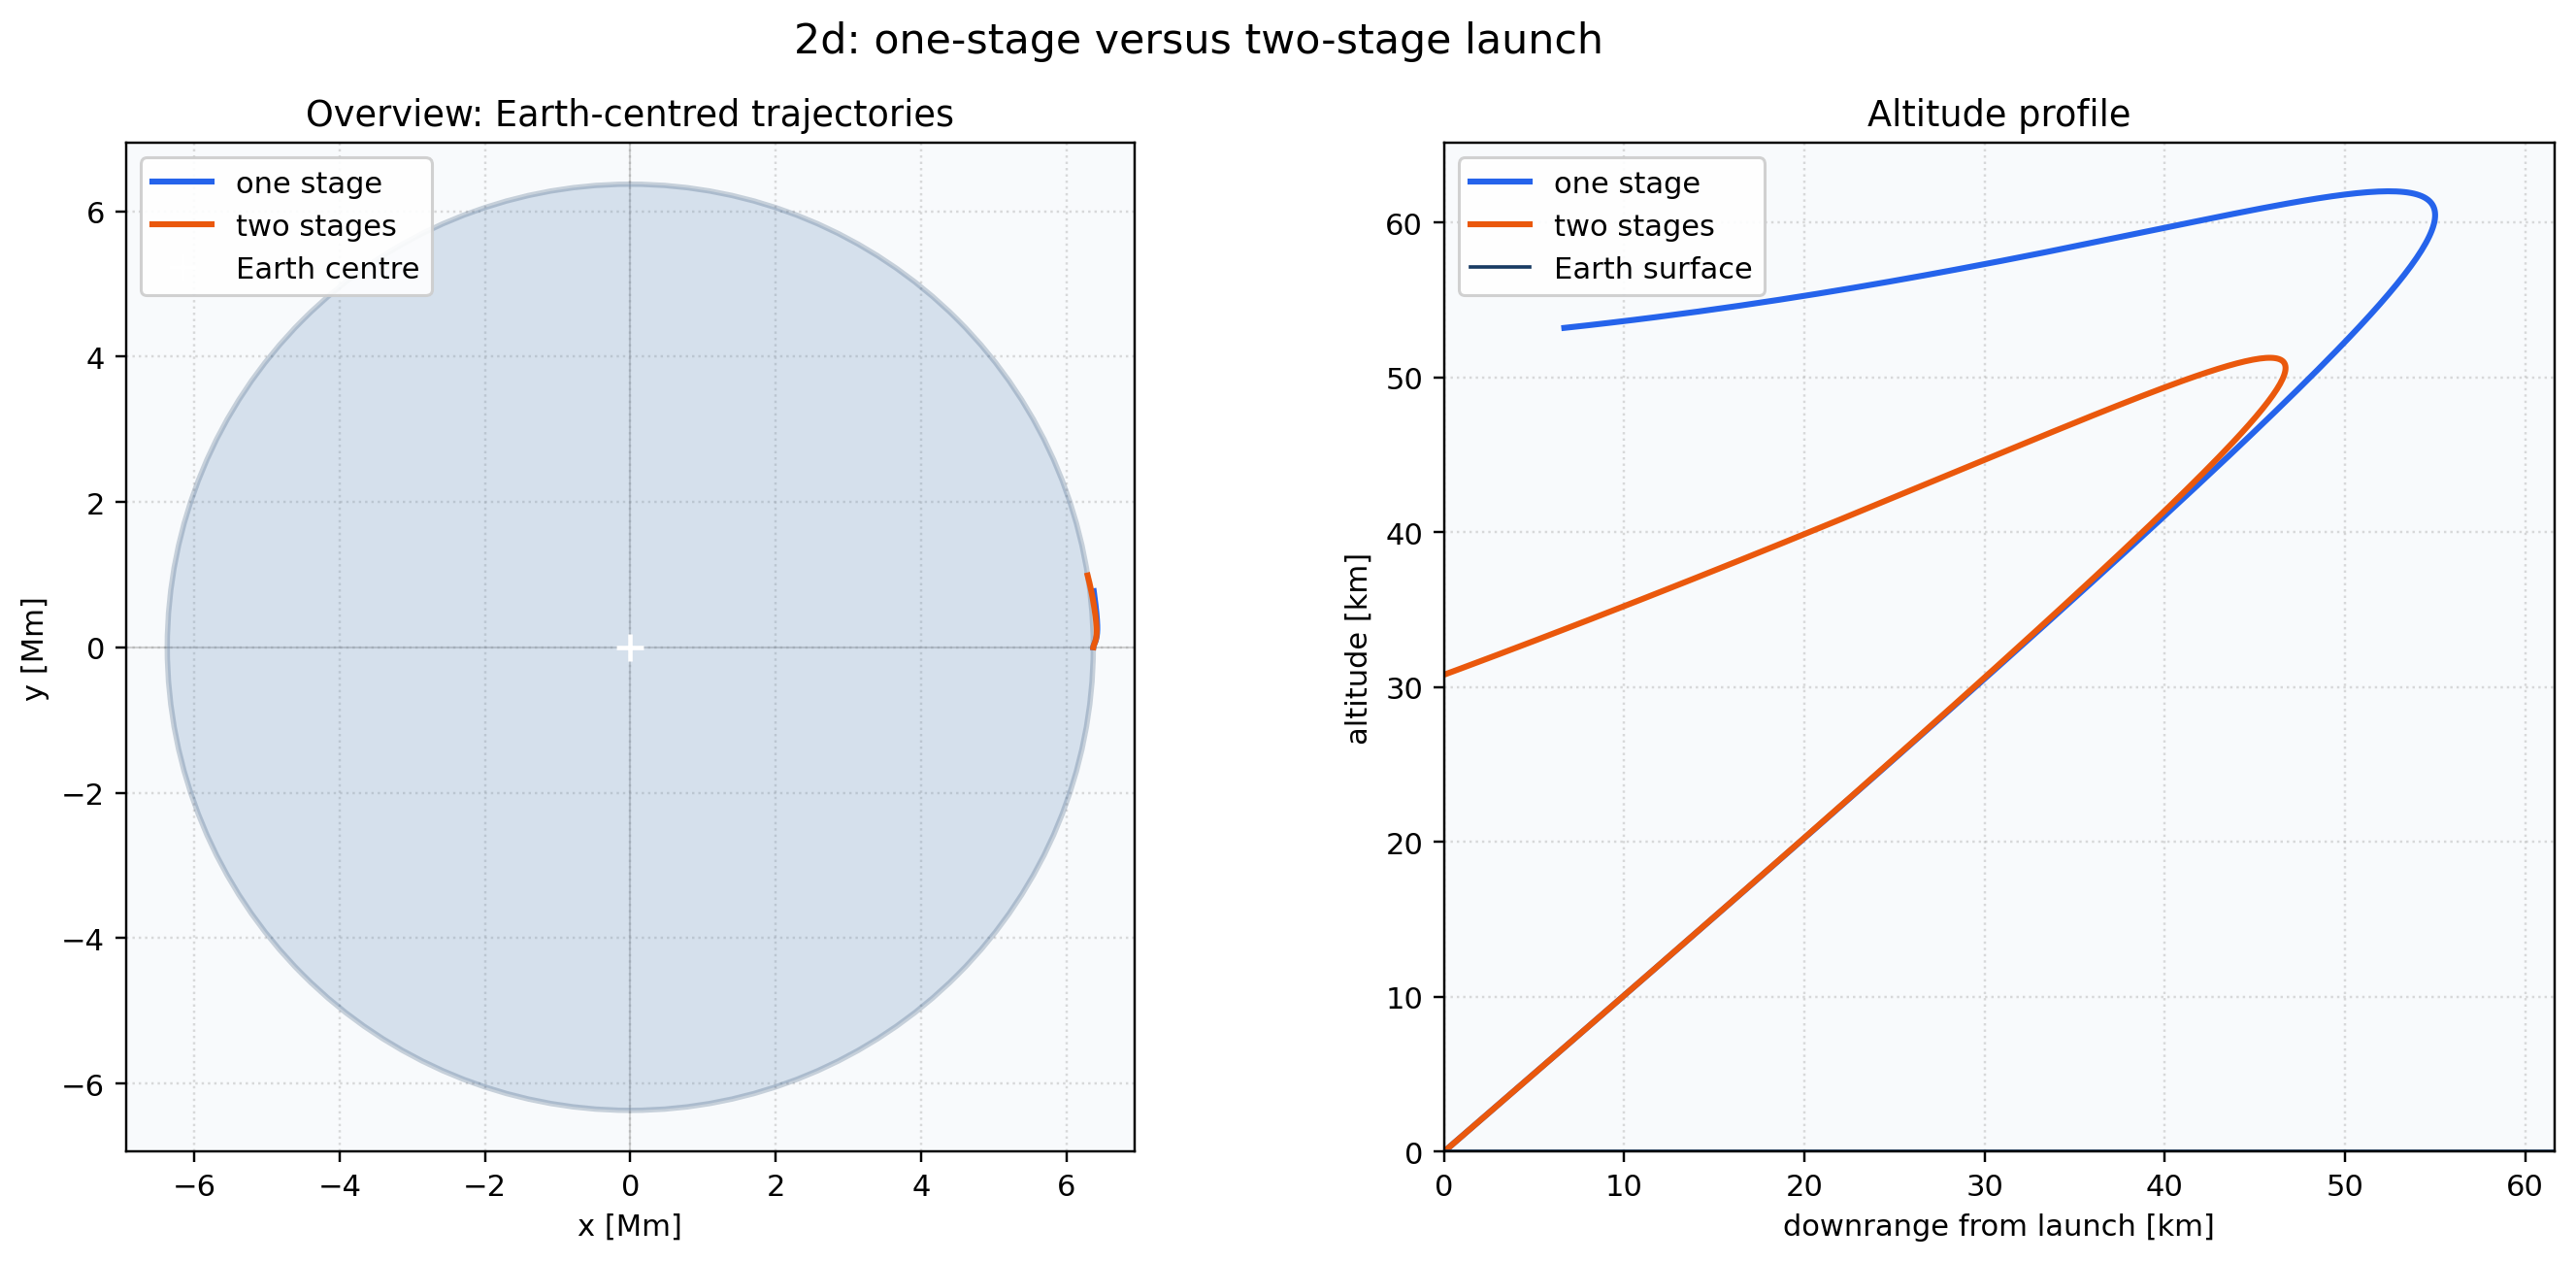
\includegraphics[width=\textwidth]{exercise_04_task_2_output/task_2d_staging.png}
\caption{Earth-centred Trajektorien und Höhenprofile der Stufenvergleiche.}
\label{fig:staging}
\end{figure}

\begin{table}[H]
\centering
\caption{Ideale Geschwindigkeitsbudgets und Simulationsstatus.}
\begin{tabular}{@{}lrrr@{}}
\toprule
Konfiguration & ideales $\Delta v$ [\si{\kilo\meter\per\second}] &
Status & $E_{\mathrm{final}}$ [\si{\mega\joule\per\kilogram}]\\
\midrule
Eine Stufe & 10.131 & überlebt Brennschluss & $-15.884$\\
Zwei Stufen & 20.263 & Absturz & $-40.770$\\
\bottomrule
\end{tabular}
\end{table}

Mit dem unveränderten $t_p=\SI{150}{\second}$-Programm schneidet die
zweistufige Testtrajektorie nach der Trennung die Erdoberfläche. Das ist kein
Widerspruch zum größeren idealen $\Delta v$: Die Flugführung wird nach der
Stufentrennung nicht neu optimiert, und ein erheblicher Anteil der möglichen
Geschwindigkeitsänderung geht durch Gravitation und ungünstige Flugrichtung
verloren. Eine realistische zweistufige Strategie würde nach der Trennung die
Schubrichtung prograd nachführen und den Zeitpunkt der Stufentrennung
optimieren.

\section{Fazit}

Die Mondaufgabe zeigt, dass für Langzeitbahnen nicht nur die lokale Ordnung
eines Verfahrens entscheidend ist. Symplektische Verfahren bewahren die
geometrische Struktur des Hamilton-Systems und liefern deshalb trotz
beschränkter Energiefehler robuste Langzeitbahnen. Die Raketenaufgabe ergänzt
dies um variable Masse, Schubsteuerung, Erdrotation und diskrete
Geschwindigkeitskorrekturen. Dort entscheidet neben dem idealen
Raketengleichungsbudget vor allem die tatsächliche Flugführung darüber, ob
eine gebundene Bahn, ein Absturz oder Flucht entsteht.

\end{document}
